\subsection{Lorenzkraft $\vec{F_L}$}
    \begin{minipage}{0.49\linewidth}
        \begin{empheq}[box = \fbox]{align*}
            \vec{F_L} &= I (\vec{l} \times \vec{B})\\
            &= \int \vec{j} \times \vec{B} dV\\
            &= \int \rho (\vec{v} \times \vec{B}) dV\\
            &= q (\vec{v} \times \vec{B})
        \end{empheq}
        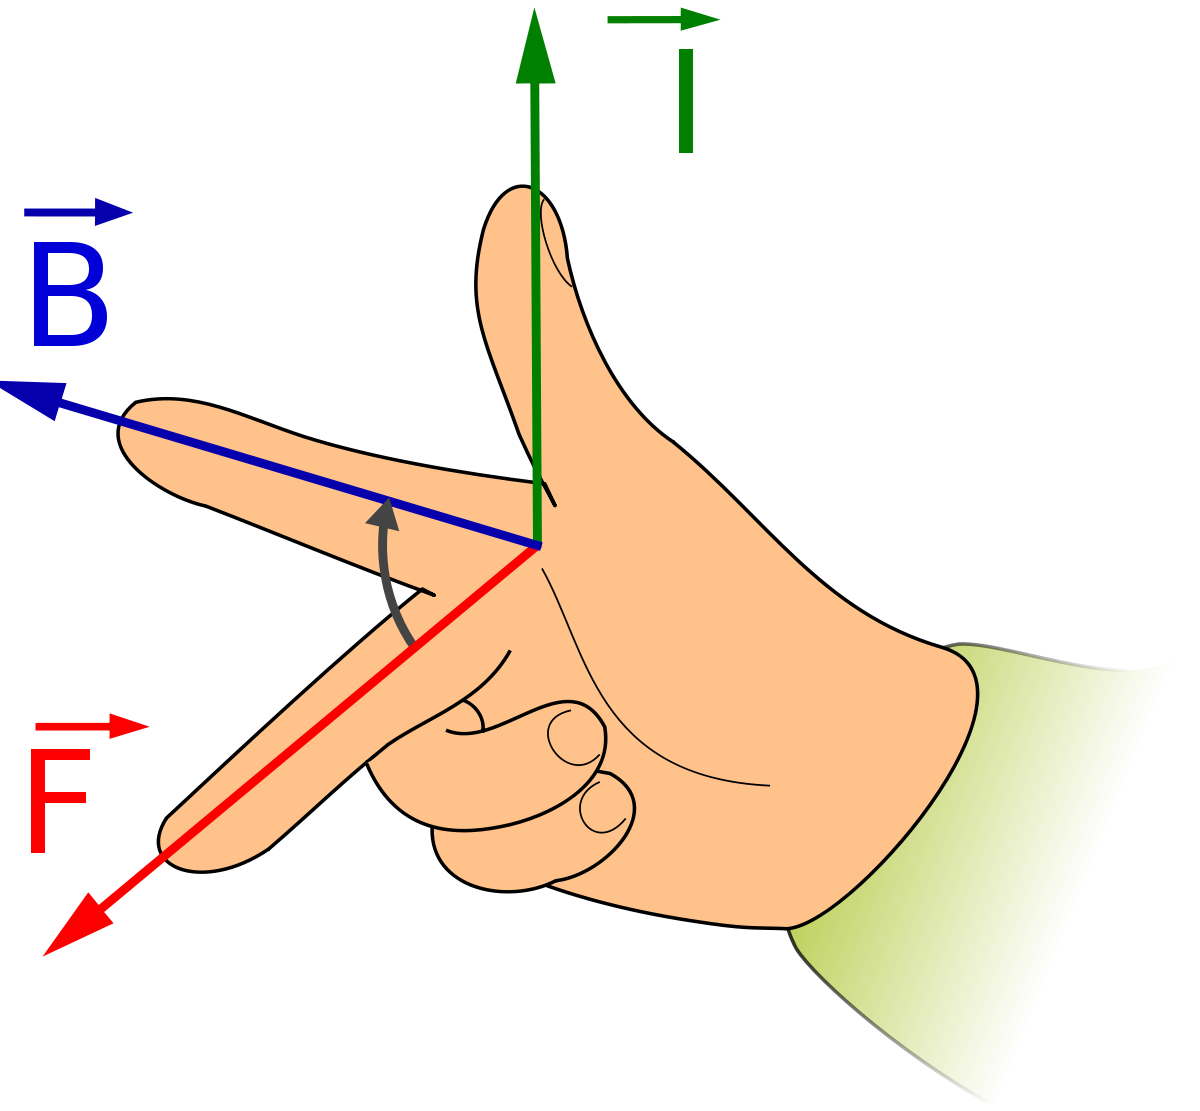
\includegraphics[width = \linewidth]{src/images/rechte_hand_lorenz.png}
    \end{minipage}
    \begin{minipage}{0.49\linewidth}
        \begin{scriptsize}
            \begin{empheq}{align*}
                l = &\text{Länge stromdurchflossener}\\
                &\text{Leiter in Magnetfeld}\\
                A = &\text{Querschnittsfläche Leiter}\\
                V = &A \cdot l = \text{Volumen Leiter}\\
                j = &\frac{I}{A} = \text{Flächenstromdichte}\\
                \rho = &\text{Volumenladungsdichte}\\
                \vec{B} = &\text{Magnetfeld}\\
                I = &\rho A v = \text{el. Strom}\\
                v = &\text{Geschwindigkeit der Ladungen}\\
                q = &\text{Ladung !Vorzeichen!}
            \end{empheq}
            \linebreak
            ACHTUNG: Elektronenfluss in entgegengesetzte Richtung zu Fluss des technischen Stroms
        \end{scriptsize}
    \end{minipage}